%%%%%%%%%%%%%%%%%%%%%%%%%%%%%%%%%%%%%%%%%%%%%%%%%%%%%%%%%%%%%%%%%%%%%%%
%%%%  Load the document class and packages                         %%%%
%%%%%%%%%%%%%%%%%%%%%%%%%%%%%%%%%%%%%%%%%%%%%%%%%%%%%%%%%%%%%%%%%%%%%%%
\documentclass[a4paper]{report}
\usepackage{epsfig}            % to insert PostScript figures
\graphicspath{ 
  {figures/} 
}

%Change figure names
\renewcommand{\figurename}{Fig}

\usepackage[bf,footnotesize]{caption} % make captions small and label bold


\addtocounter{chapter}{1} %Because starting at zero is silly
\makeatletter
\renewcommand{\thesection}{\@arabic\c@section}
\renewcommand{\thefigure}{\@arabic\c@figure}
\makeatother

\usepackage[a4paper,margin=2.7cm,tmargin=2.5cm,bmargin=2.5cm]{geometry} 
\usepackage{textcomp}          % To make nice degree symbols and others\usepackage[bf,footnotesize]{caption} % make captions small and label bold
\usepackage{wrapfig}
%to produce the clickable references along the left in Acroread. This
%package must be included last. 
\usepackage[ps2pdf,bookmarks=TRUE]{hyperref} 



\usepackage{wasysym}





%%%%%%%%%%%%%%%%%%%%%%%%%%%%%%%%%%%%%%%%%%%%%%%%%%%%%%%%%%%%%%%%%%%%%%%
%%%%  Hypertext references for Acrobat                             %%%%
%%%%%%%%%%%%%%%%%%%%%%%%%%%%%%%%%%%%%%%%%%%%%%%%%%%%%%%%%%%%%%%%%%%%%%%
\hypersetup{
pdfauthor = {SWC},
pdftitle = {Optics Exercises},
pdfkeywords = {optics, lenses, refraction, reflection, dispersion,
  telescope, microscope},
pdfcreator = {LaTeX with hyperref},
pdfproducer = {dvips + ps2pdf}
           }


\begin{document}




%set the number of sectioning levels 
\setcounter{secnumdepth}{2}

\begin{center}
\textbf{\Large{Optics Bench Exercises: Illuminating the Sample}}
\end{center}

\section{Introduction}
One of the key challenges of microscopy is to adequately illuminate the sample. 
By this we mean that the sample should be illuminated uniformly and from a suitably wide range of angles. 
Different samples are best illuminated in different ways.
In transmission microscopy, the sample is illuminated from the opposite side to which it is imaged. 
In fluorescence microscopy, the sample is illuminated from the same side, with the objective also serving as the condenser. 
It is not efficient to illuminate the sample directly (with no intervening lenses) because light is emitted in all directions from the source but only a narrow range of ray angles reach the specimen. 
In the following exercises you will build two different illumination systems: critical and K\"{o}hler. 


\subsection{Critical illumination of a sample}
In critical illumination the light source is focused onto the specimen (Fig.~\ref{critIlum}).
This provides illumination from a range of angles but has a major drawback which will become apparent soon. 
You will first you will set up critical illumination with one lens.

\begin{figure}[h]
\center
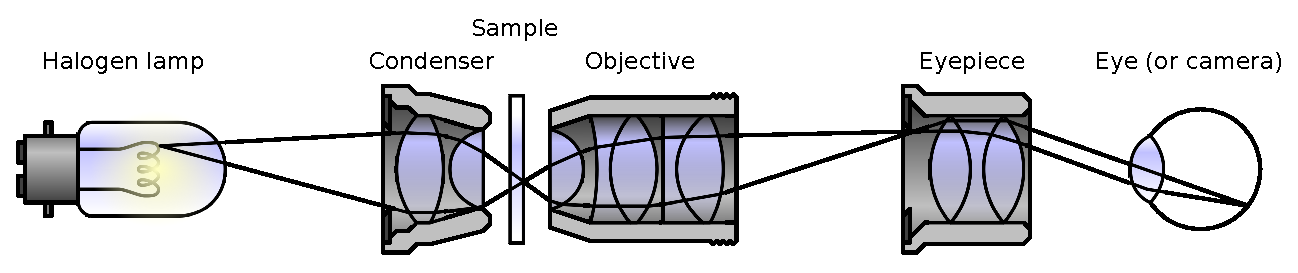
\includegraphics[width=5in]{Critical_Illumination.eps}
\caption{A simple critical illumination set up for visual microscopy.}
\label{critIlum}
\end{figure}


Set the laser at one end of the rail and align the beam with the rail using a single iris:
\begin{itemize}
    \setlength\itemsep{0.1em}
    \item Set the iris to a height suitable for adding 2'' optics. You can mount the iris to a $75~mm$ post and use a $50~mm$ post holder. 
    \item Clamp the laser pointer to one end of the rail.
    \item With the iris next to the pointer, \textit{translate} the pointer until it goes through the iris. 
    \item Slide the iris to the other end of the rail and \textit{rotate} the pointer until it goes through the iris. 
    \item Repeat until the beam is parallel with the rail. 
    \item Do not translate the iris on its post to achieve beam alignemnt. 
\end{itemize} 

\begin{figure}[h]
\center
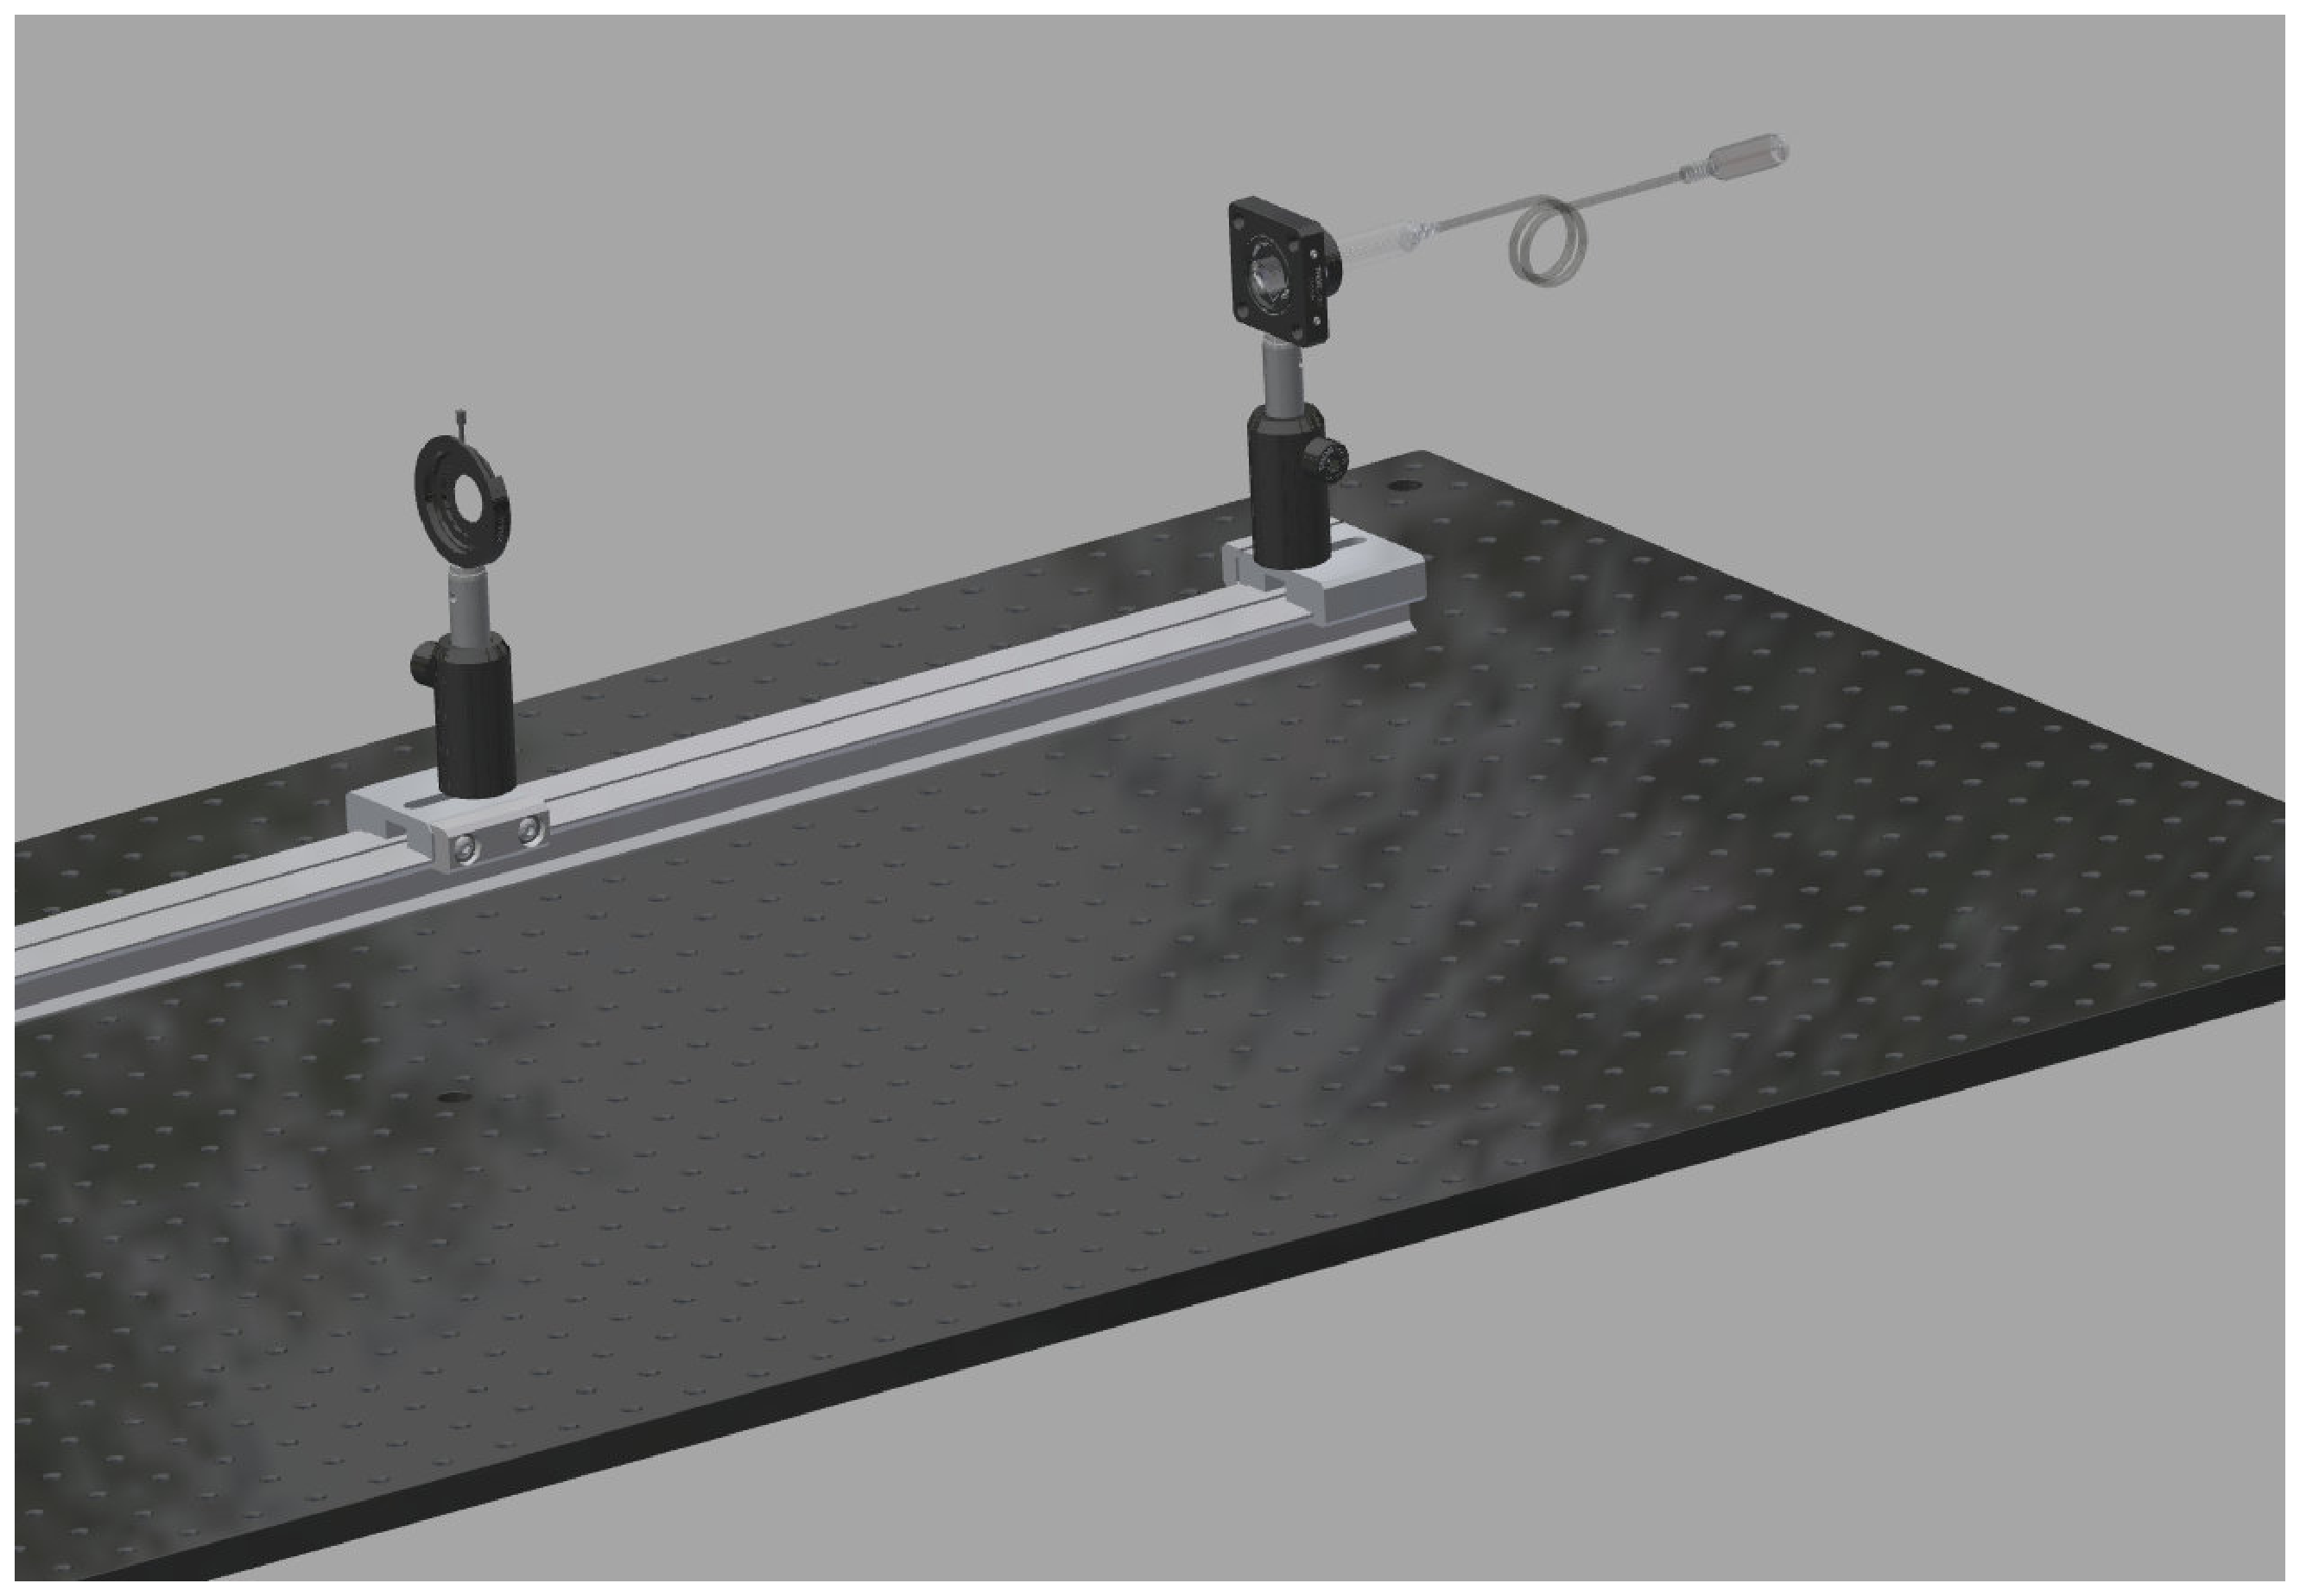
\includegraphics[width=3in]{iris_and_laser.eps}
\caption{Aligning a laser beam to the rail using an iris.}
\label{fig:beam_iris}
\end{figure}

\clearpage


Once you're done, place a positioning collar around the iris post so you can retain its height even if you have to remove it from the post holder. 
You will now align the tube lens and objective with the beam (Fig.~\ref{fig:beam_obj_tube}). 

\begin{itemize}
\item Slide the iris to the end of the rail. 
\item Place the $f=300~mm$ lens $1f$ from the iris and adjust it until the beam goes through the iris. This is your `tube lens'.
\item Place the objective upstream of the tube lens and align it such that the beam (now expanded) again goes through the iris. 
\end{itemize}

\begin{figure}[h]
\center
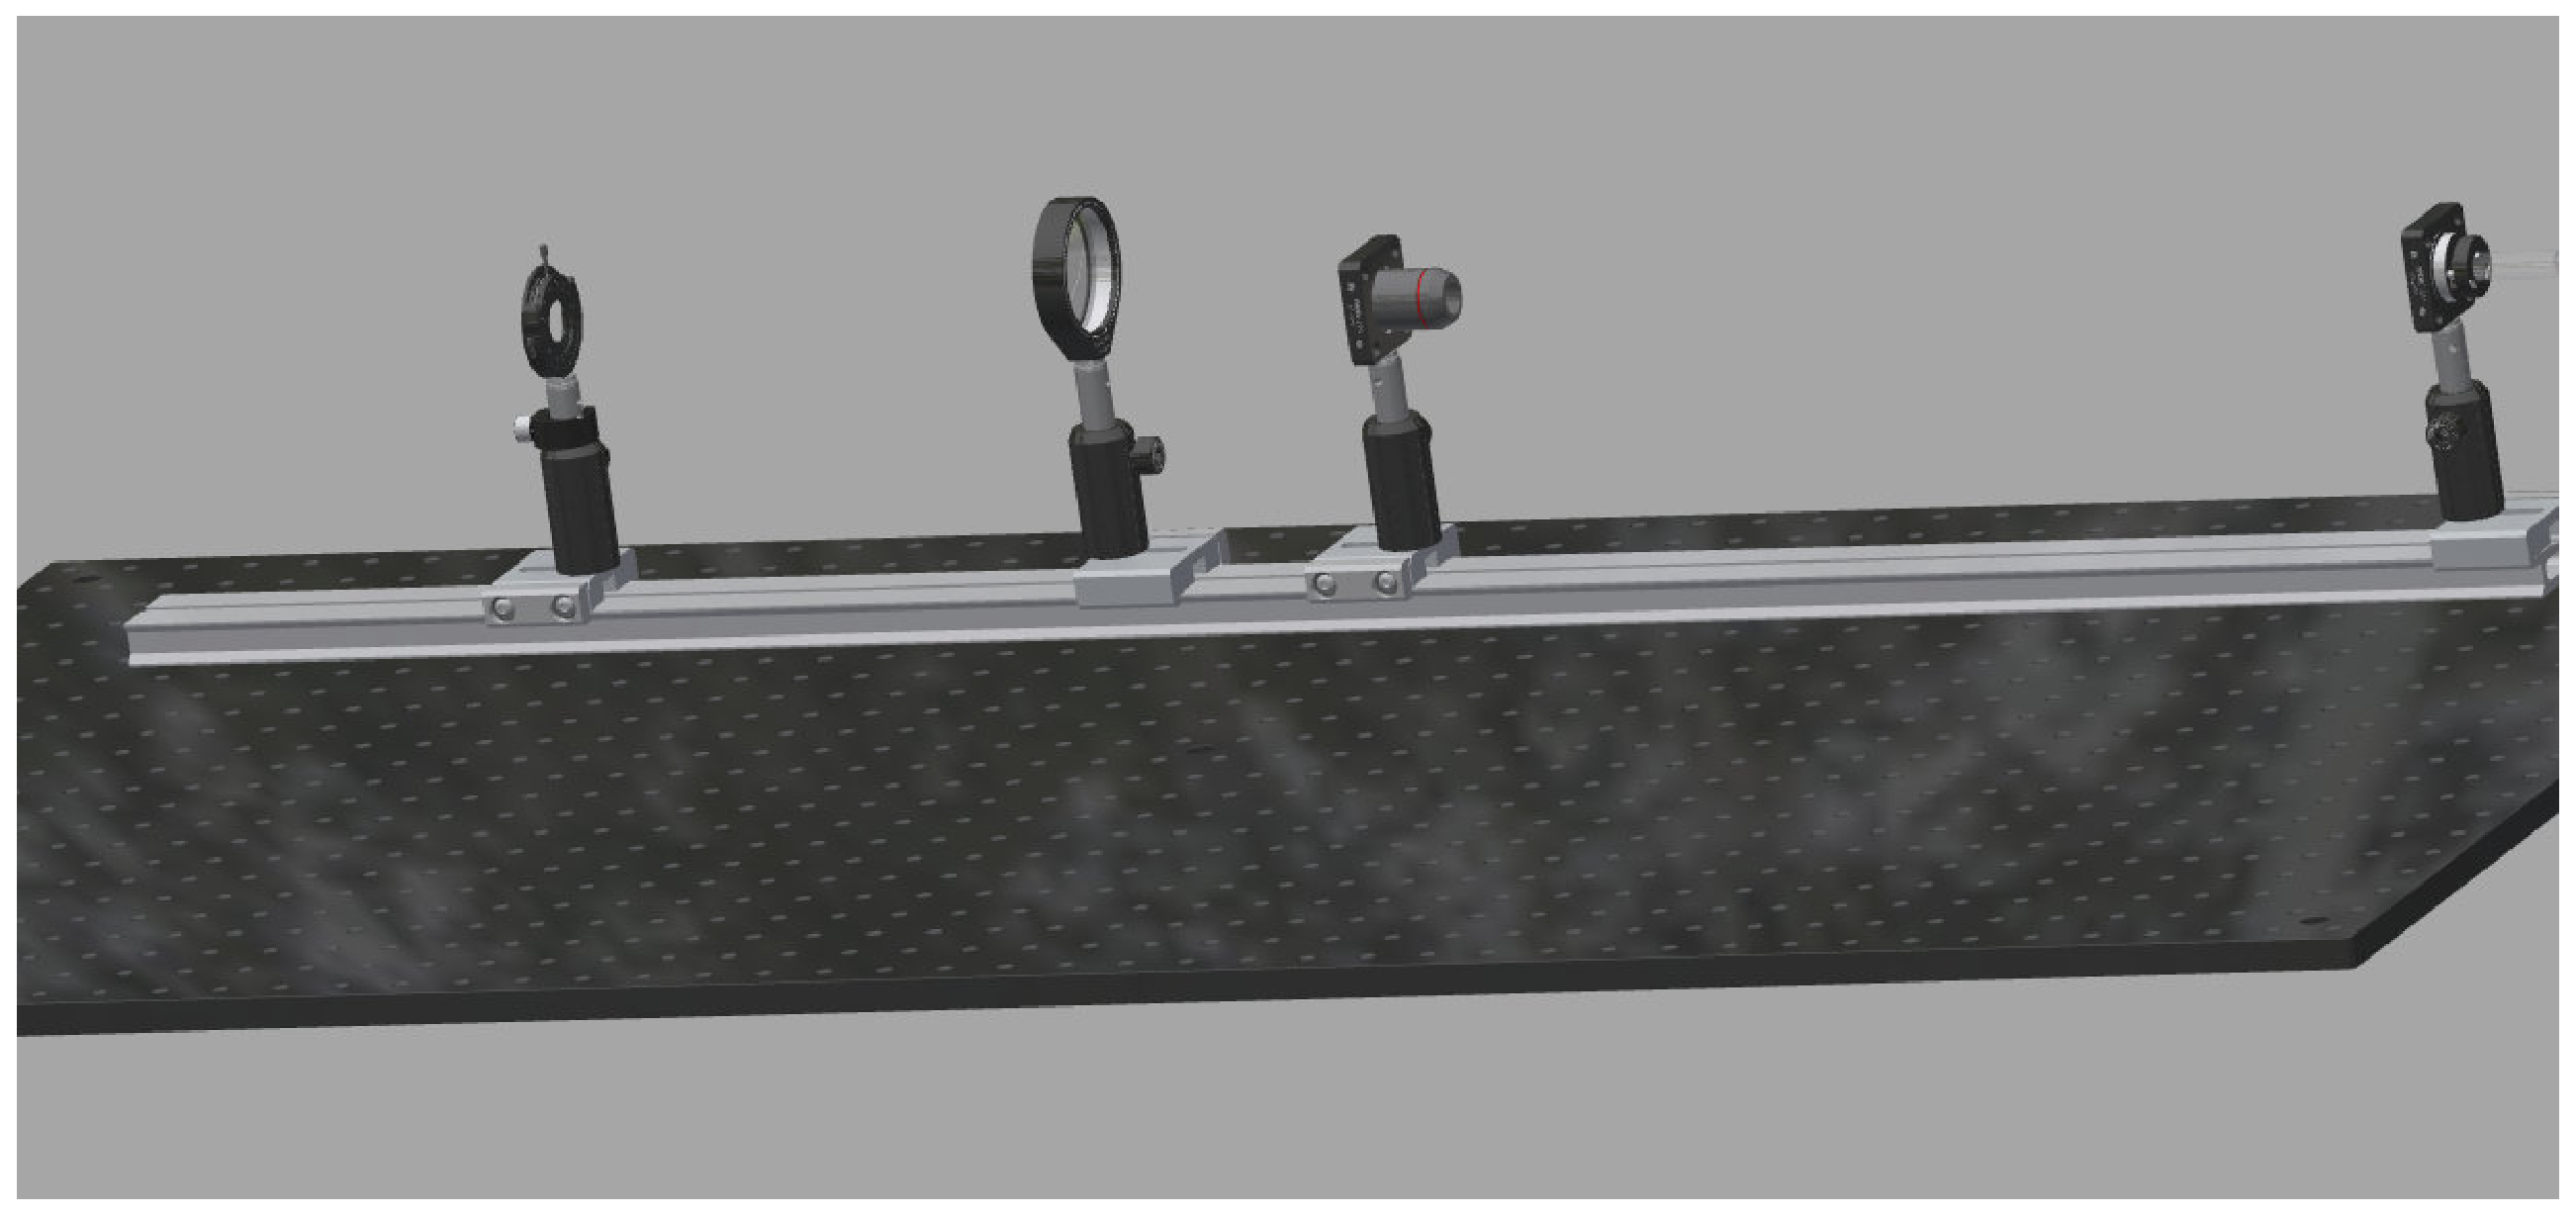
\includegraphics[width=3in]{Obj_alignment_before.eps}
\caption{Aligning the tube lens and objective with the beam.}
\label{fig:beam_obj_tube}
\end{figure}

All that is left is to add a sample, collector lens and a light source. 

\begin{itemize}
\item Hint: to avoid running out of $50~mm$ posts in the exercise that follows, use $30~mm$ or $40~mm$ posts for the 2'' lenses, sample holder, and card holder.
\item Place the light source at one end of the rail and then put a 1''{\diameter} $f=25~mm$ or $f=35~mm$ lens at $2f$ from it.
\item Place your sample at $2f$ on the other side, where the image of the LED emitter is formed.
\item Move the slide back and forth along the rail until an image of the LED emitter appears on it.
\item Place the 4x objective after the slide. This objective has a working distance of about $20~mm$.
\item At the other end of the rail, place a viewing screen onto which you will form an image.
\item Position an $f=200~mm$ lens $1f$ from the card. This is known as the tube lens and will image the sample onto the card
\footnote{The $f=200~mm$ lens will yield 4x. You could use the $f=300~mm$ lens if you wish, to yield 6x.}.
\item Move the objective back and forth a small distance to focus and obtain an image. 
\end{itemize}

The above arrangement is a simple microscope. 
As you might expect, the image of the sample also contains an image of the light source. 
This is obviously not ideal.
Before we go on to address this problem, let's improve the illumination by capturing more of the light from the source. 
The plan is as follows (don't build it yet):
We will add an 2''{\diameter} $f=60~mm$ before the sample, forming an infinite conjugate system with the existing lens. 
The lens nearer the source is known as the \textbf{collector lens} and will be at $1f$ from the source.
The lens nearer the sample is known as the \textbf{condenser lens} and is at $1f$ from the sample. 
This is still critical illumination, since the light source will be imaged onto the sample, but the collector lens will be closer to the source and so more light will be captured. We will align the lenses with the laser pointer:

\begin{itemize}
\item Remove all the posts (not the rail carriages) from the rail.
\item Add all 10 post and rail carriage assemblies to your rail. You will need 6 carriages between the objective and the light source.
\item Replace the light source with the laser pointer on a $75~mm$ post. 
\item Use an iris as before to align the beam. However, this time you will have to move it between post holders and maintain its height with a post collar since you won't be able to slide it along the rail.
\item Replace the tube lens and position it at the same height as the beam. Use the iris to help you.
\item Add objective upstream of the tube lens. Get the laser beam hitting the middle of the of front element. 
\item Now place the iris in the specimen's post holder and locate the $f=60~mm$ condenser lens next to it, using the iris as a target. 
\item Replace the iris with the sample
\item Use the iris to place the $f=30~mm$ collection lens in front of the laser.
\item Leave the iris where it is but open it. 
\item \textbf{You should have two empty carriages between the iris and the condenser lens}
\item Replace the laser pointer with your light source. 
\item Move the lenses back and forth so as to obtain a focused image under critical illumination. 
\end{itemize}


With an infinite conjugate illumination system it becomes possible to regulate the NA of the illumination by varying the size of the iris in the infinite space. 
Try it!
By altering the NA of the illuminated light, the iris provides control over the resolution, contrast, and depth of field (Fig.~\ref{fig:critical_iris}).
To see the effect: open the iris, defocus slightly by moving the objective, now close the iris. The image will go back into focus. 

\begin{figure}[h]
\center
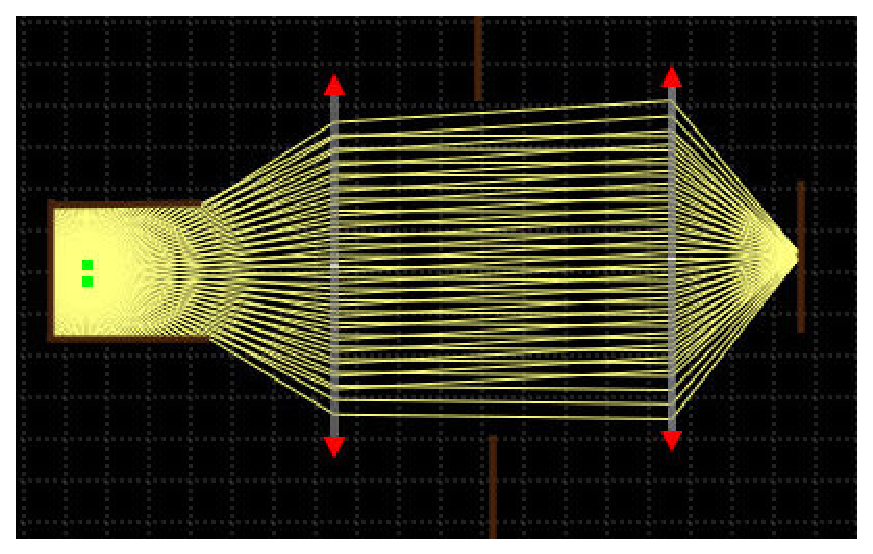
\includegraphics[width=2.8in]{critical_open_iris.eps}
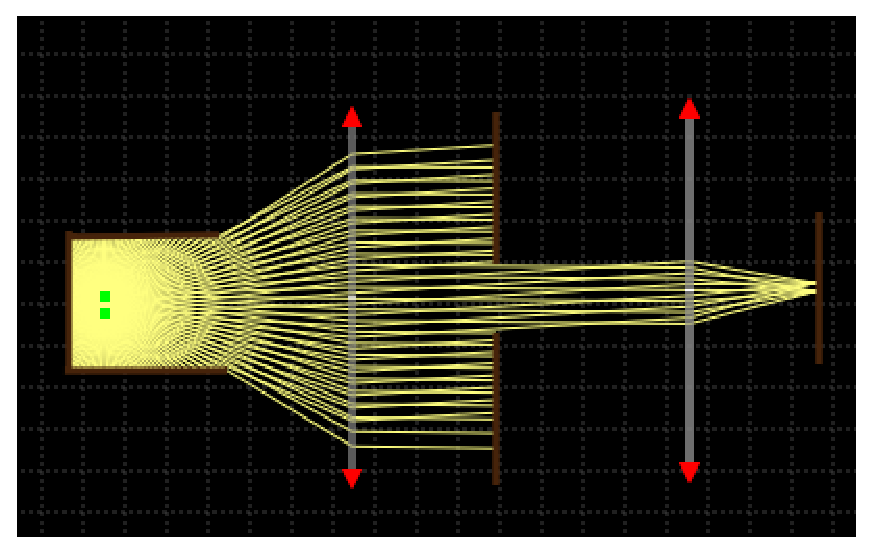
\includegraphics[width=2.8in]{critical_closed_iris.eps}
\caption{Critical illumination with two lenses. 
There is an iris after that collector lens that is open on the left image and closed on the right image. 
Note how closing the iris restricts the range of angles reaching the sample.}
\label{fig:critical_iris}
\end{figure}



\clearpage

\subsection{K\"{o}hler Illumination}
K\"{o}hler illumination is an important and commonly used technique in light microscopy, as it provides even illumination of the sample whilst ensuring the light source (e.g. the bulb filament) is not visible. 
This is achieved by adding a third lens, the field lens, before the condenser so that the image of the light source is out of focus at the sample. 
Since the source is out of focus, the illumination is uniform. 
Instead, the image is formed at $1f$ from the field lens. 
The condenser is then located at $1f$ from this image (as in a beam expander) so collimated (i.e. out of focus) light reaches the sample. 

The key to understanding K\"{o}hler illumination is to consider the two sets of conjugate planes in the system (Fig.~\ref{fig:koehler}). 
The \textbf{sample} is, of course, conjugate with the image plane but it also conjugate with a point $1f$ from the collector lens ($f_{CL}$ in Fig.~\ref{fig:koehler}). 
The \textbf{light source} is conjugate with a location between the field lens and the condenser ($f_F$ and $f_{CO}$ in Fig.~\ref{fig:koehler}). 
The light source is also conjugate with the objective back aperture (not shown in Fig.~\ref{fig:koehler}). 

\begin{figure}[ht]
\center
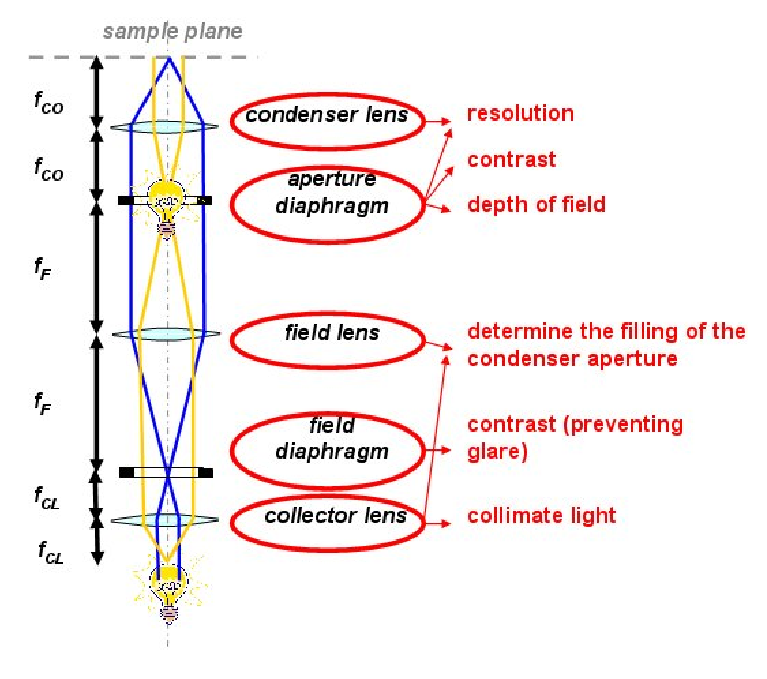
\includegraphics[width=5in]{koehler.eps}
\caption{K\"{o}hler Illumination. 
The blue lines indicate the conjugate relationship between the sample plane and the location of the field diaphragm.
The yellow lines indicate the conjugate relationship between the light source plane and the location of the aperture diaphragm.
}
\label{fig:koehler}
\end{figure}

At the the two conjugate planes in the illumination path are two irises (diaphragms). 
The \textbf{field diaphragm} is at $1f$ before the field lens, in the point conjugate with the sample. 
The field lens and condenser lens form an infinite conjugate system that image the field diaphragm onto the sample. 
The field diaphragm appears in focus at the sample and is used to regulate the area of illumination. 
This helps to improve contrast by minimizing stray light. 
Remember, the The \textbf{f}ield planes are the image \textbf{f}orming planes. 

The \textbf{aperture diaphragm} is located in the plane conjugate with the light source. 
i.e. it is located where an image of the light source is formed. 
Opening and closing this diaphragm regulates which regions of the light source can contribute to the illumination. 
Closing the diaphragm blocks off-axis regions of the light source and stops them from generating the more oblique rays that come out of the condenser. 
Closing the aperture diaphragm reduces the NA of the illumination and increases depth of field. 

\clearpage

You will now convert the critical illumination to K\"{o}hler illumination simply by adding the $f=60~mm$ field lens and an extra iris.
The components will be arranged in the following order and are all at $1f$ from each other (Fig.~\ref{fig:koehler}):
\begin{enumerate}
\setlength\itemsep{0.1em}
\item Collector lens
\item Field diaphragm.
\item Field lens ($f=60$)
\item Aperture diaphragm
\item Condenser lens ($f=60$)
\item The objective and tube lenses as before.
\end{enumerate}

The completed arrangement of the components is shown in Fig.~\ref{fig:koehler_completed}. 
Build the K\"{o}hler setup and observe that the image of the emitter is gone. 
You will likely need to tweak the distances between the components to get the field diaphragm conjugate with the sample. 
Once this is done, regulate the size of the field diaphragm and observe the effect. 
Defocus slightly and close the aperture diaphragm. Observe the effect.
You have finished! Unfortunately, the princess is another castle. See you tomorrow. 

\begin{figure}[h]
\center
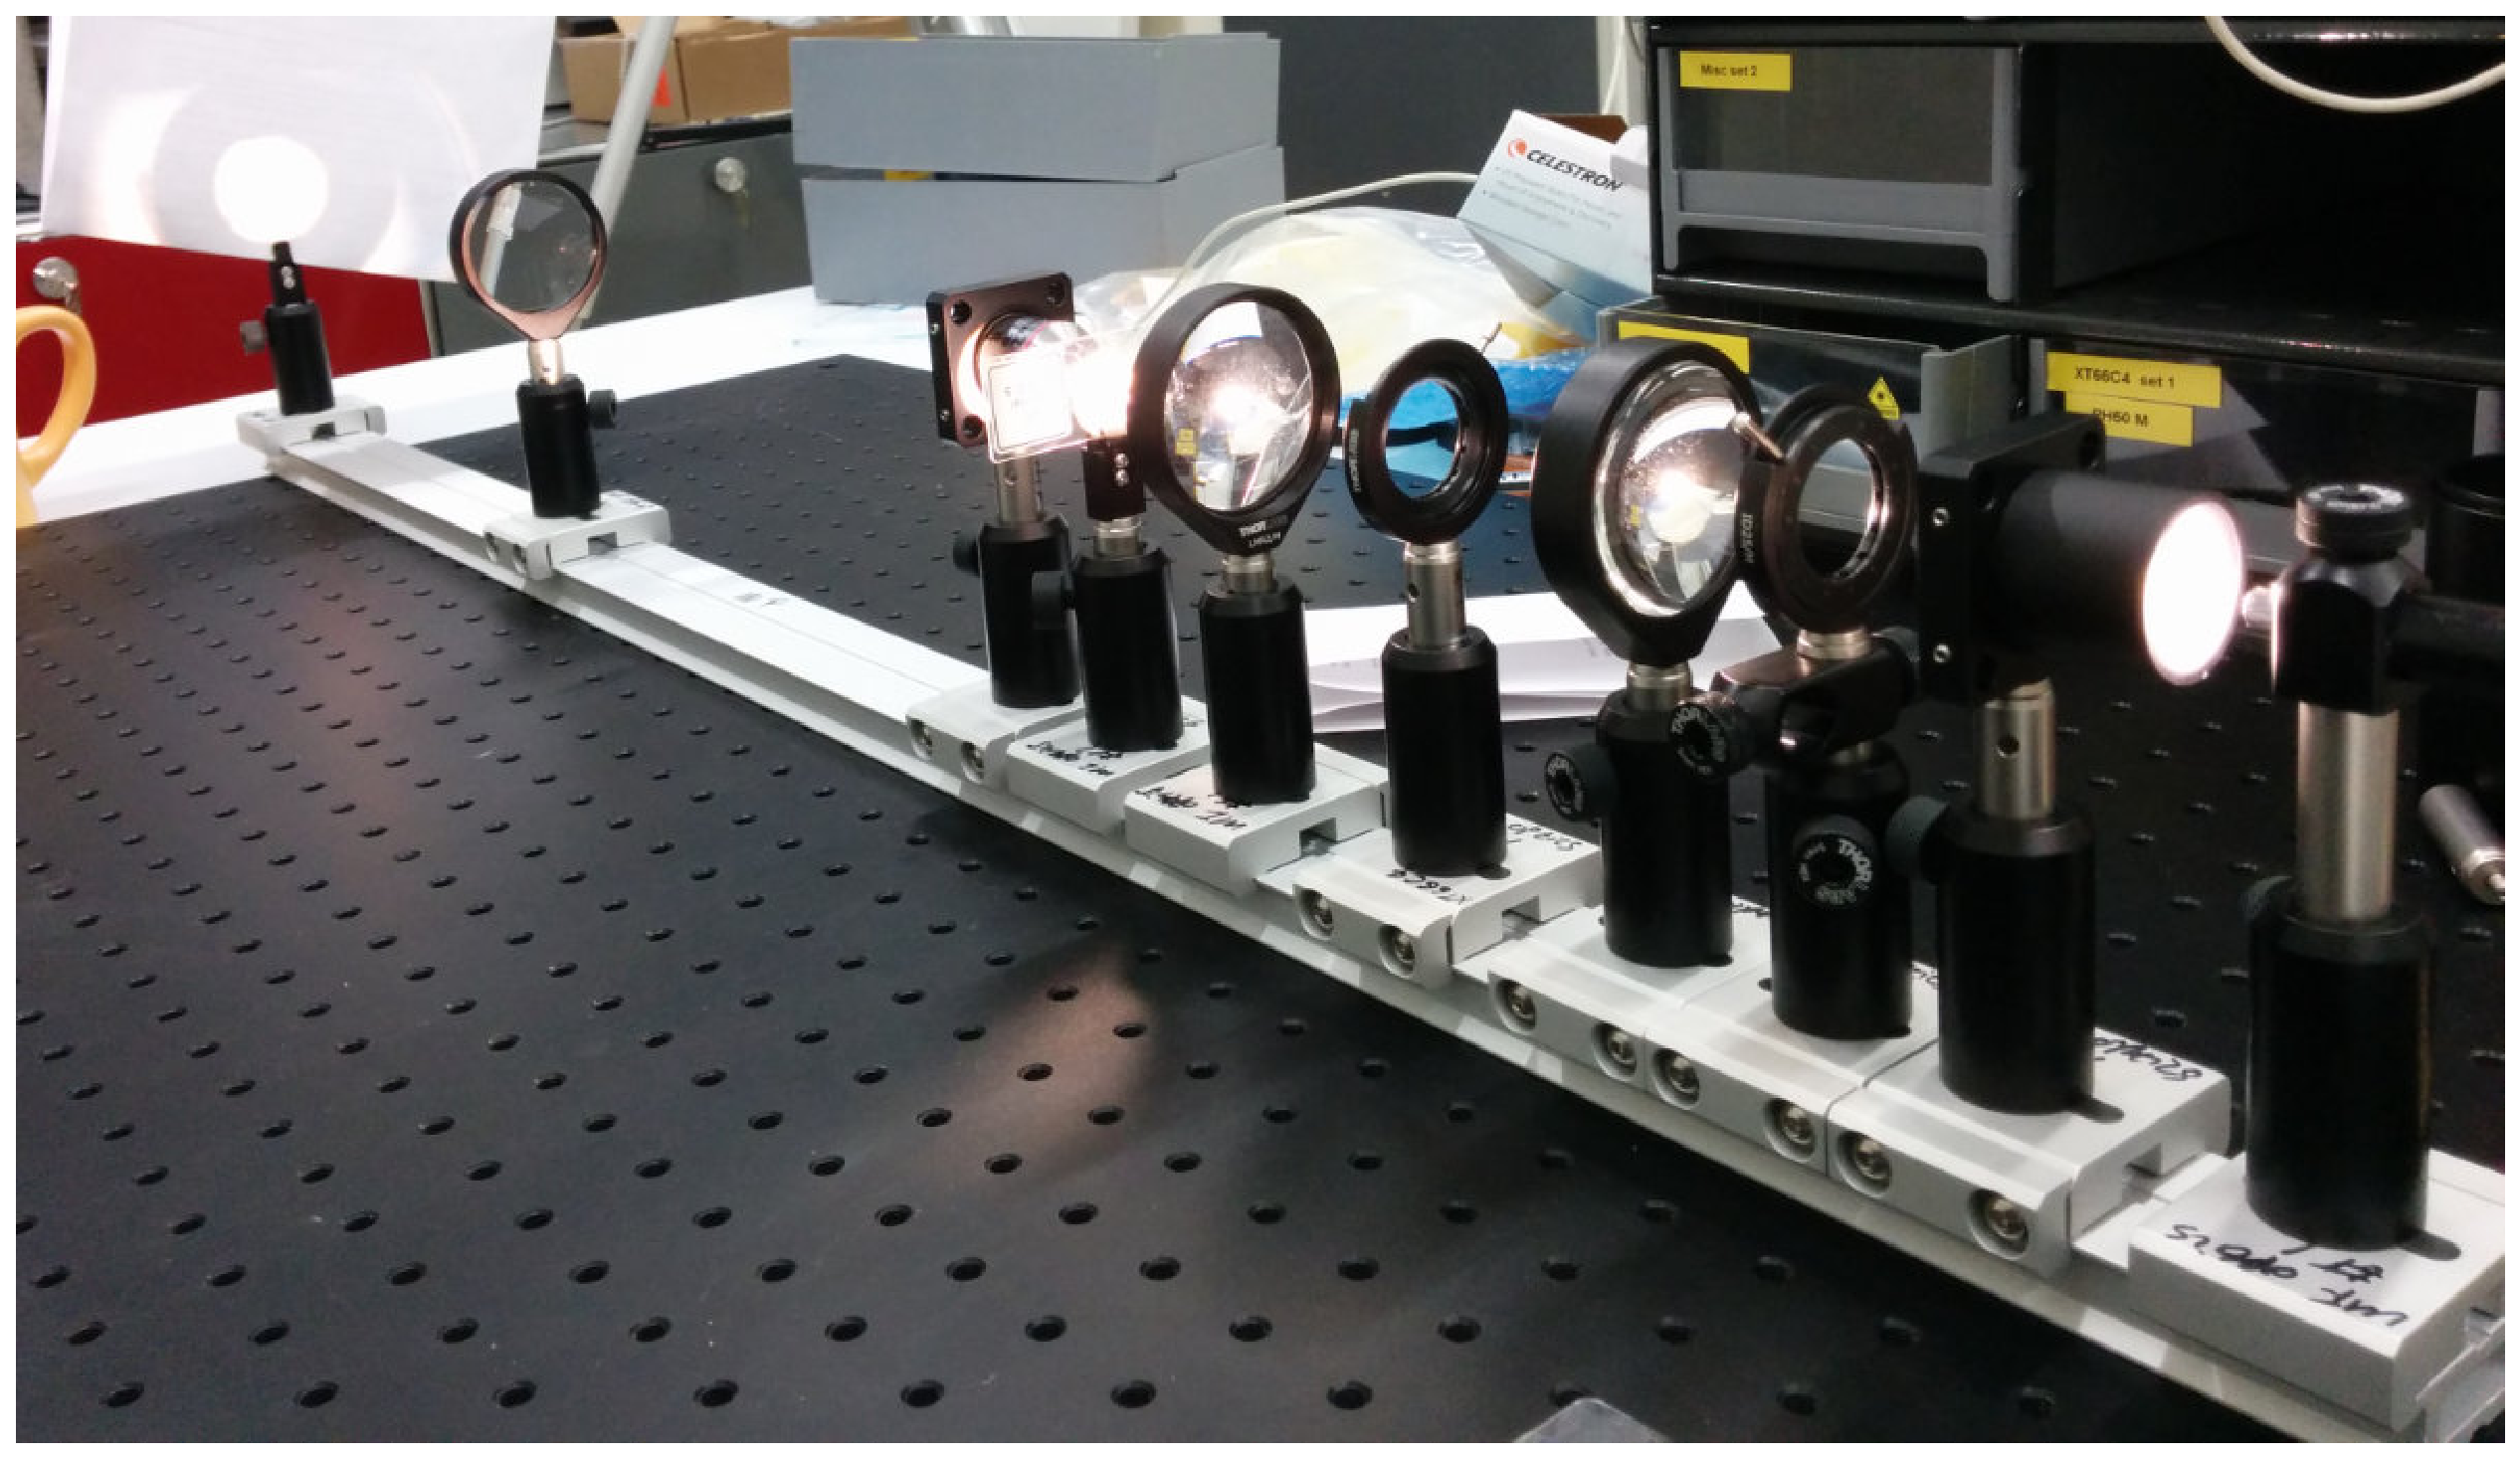
\includegraphics[width=5.5in]{illum_complete.eps}
\caption{The completed K\"{o}hler illumination assembly on a rail.}
\label{fig:koehler_completed}
\end{figure}






\end{document}
